\subsection{Comparison of the two methods}
\label{subsec:comparison_of_the_two_methods}

As we can see from Figure \ref{fig:static_responses}, the two methods give the same results.
This is expected, as in fact, the acceleration approach is just a derivation of the displacement approach, since the mass matrices $M$ and the stiffness matrices $K$ are just an implementation of the displacement and or the force method used to solve structures.

\begin{figure}[H]
    \centering
    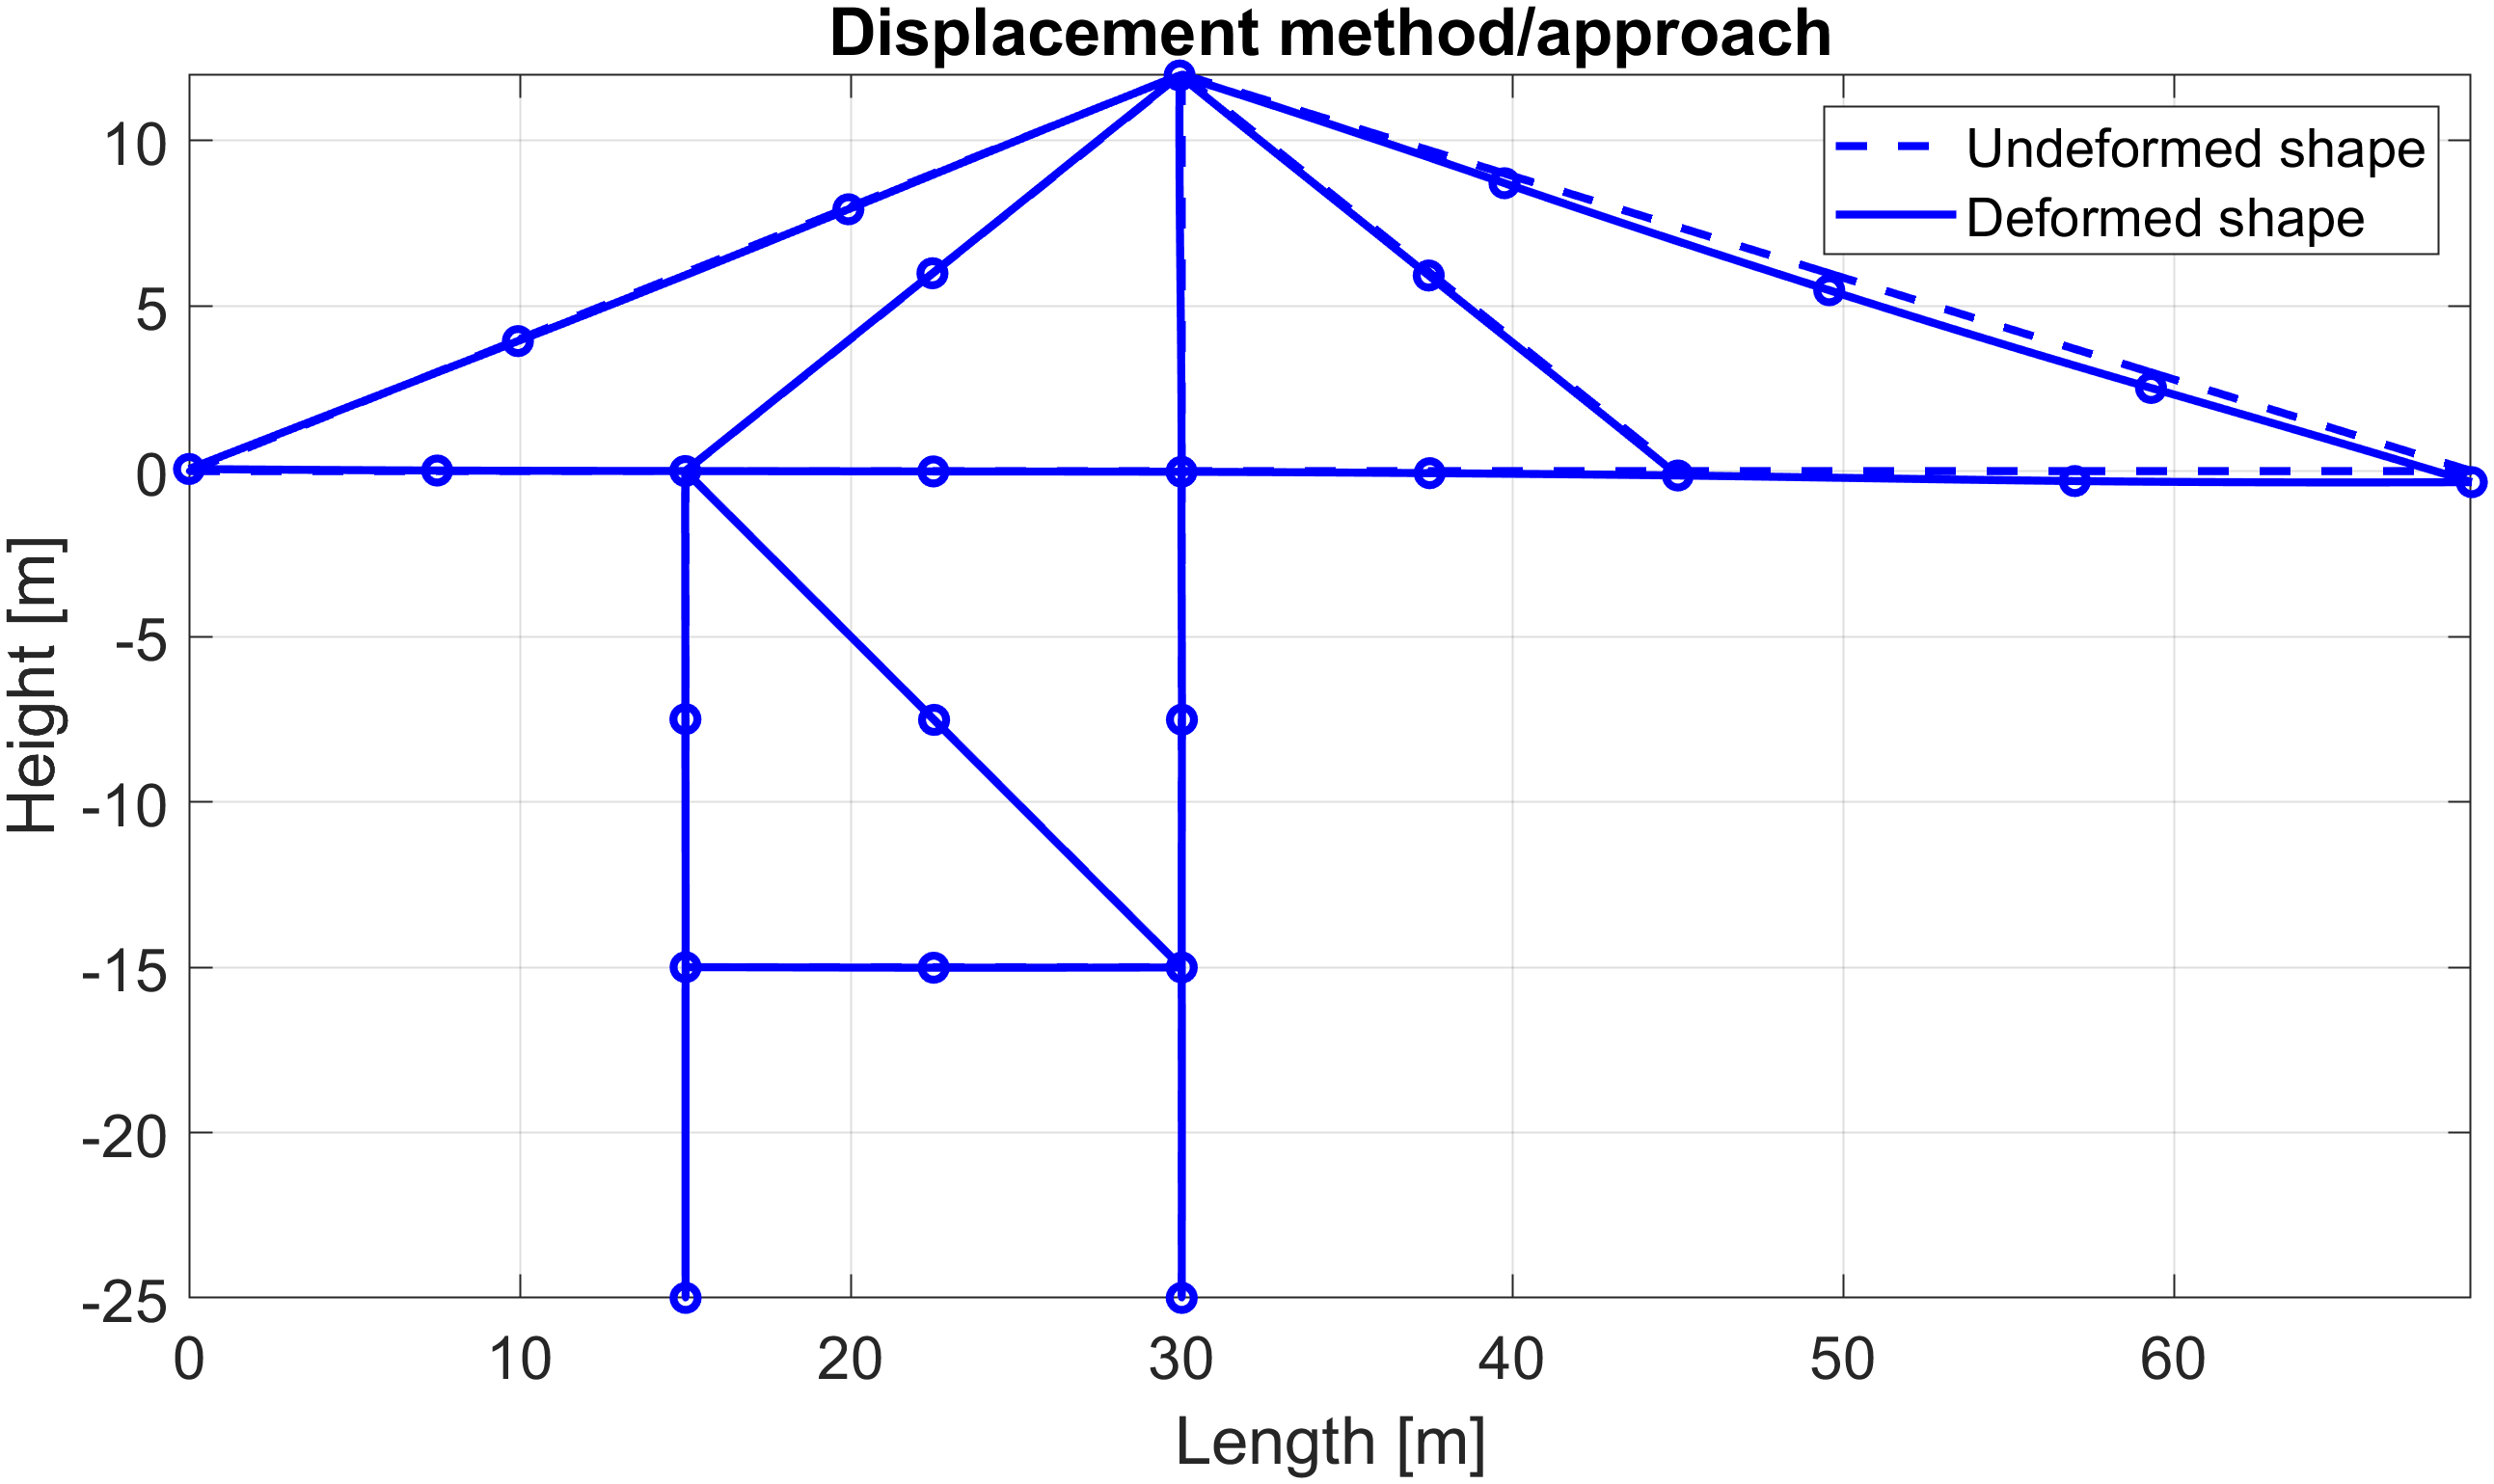
\includegraphics[width=0.45\textwidth]{img/MATLAB/Responses/Gravity_displacement.png}
    \hfill
    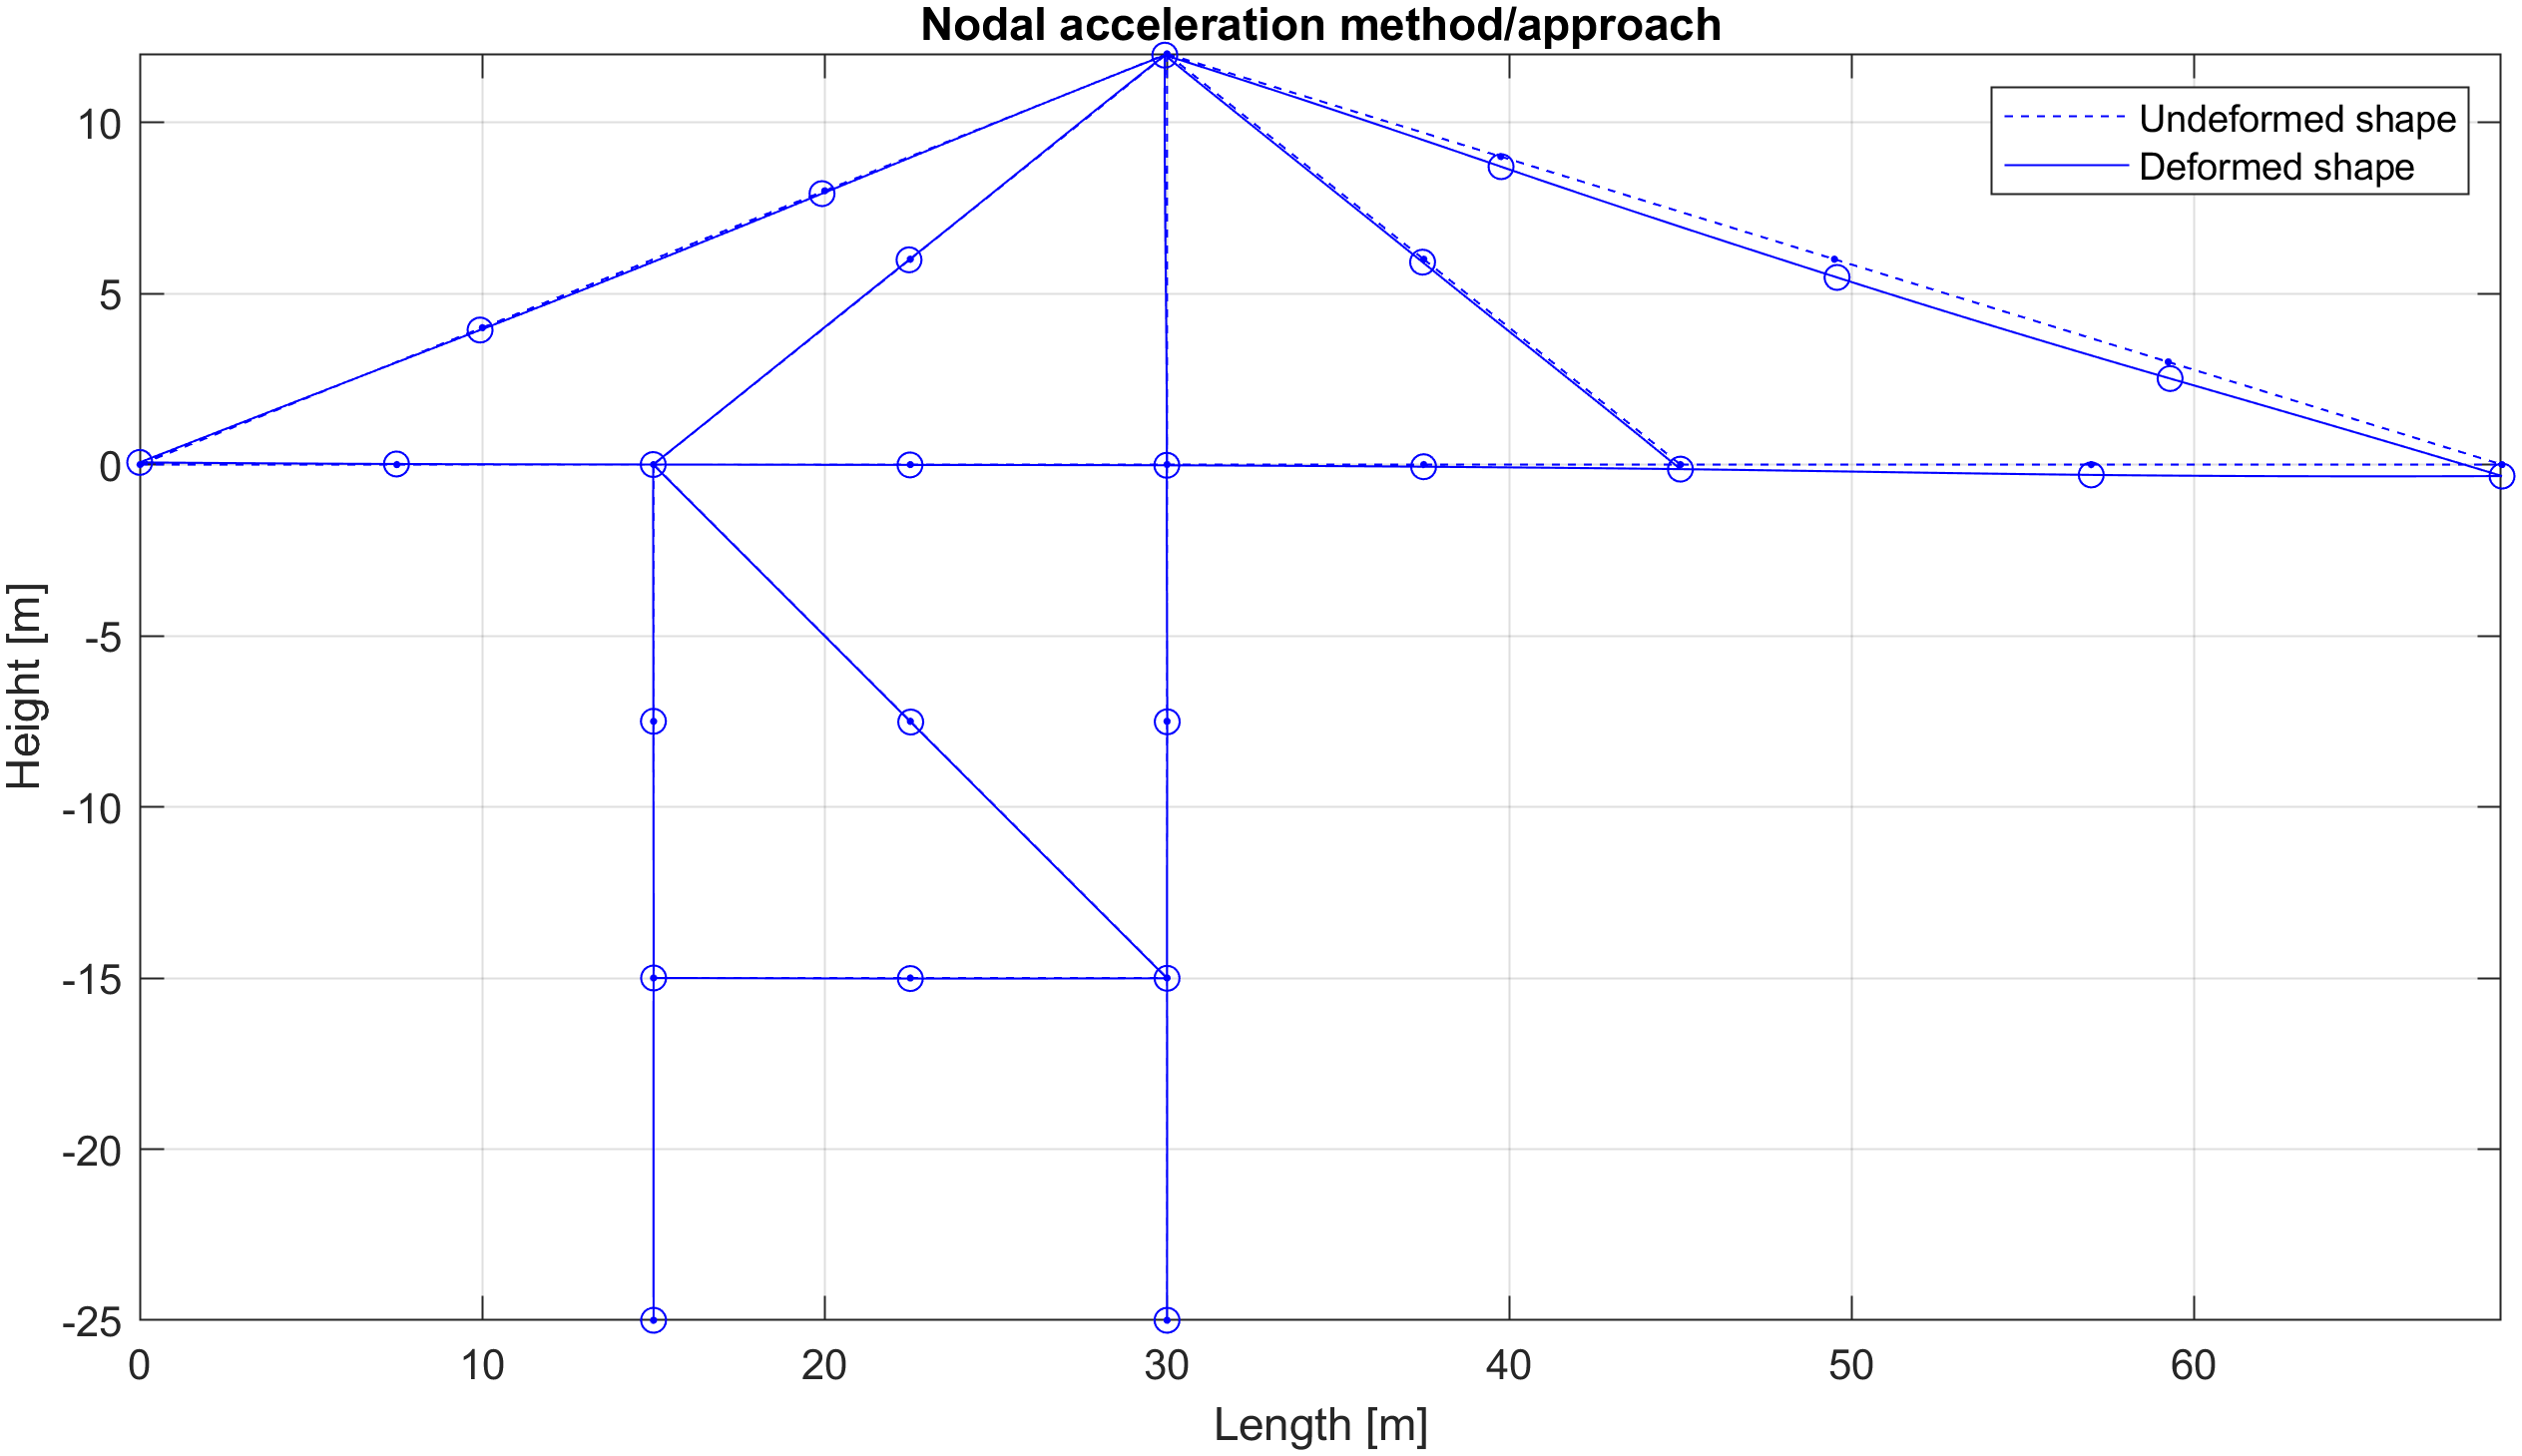
\includegraphics[width=0.45\textwidth]{img/MATLAB/Responses/Gravity_acceleration.png}
    \caption{Comparison of the static responses of the structure computed using the displacement approach and the acceleration approach.}
    \label{fig:static_responses}
\end{figure}